\begin{figure*}[t]
\begin{center}
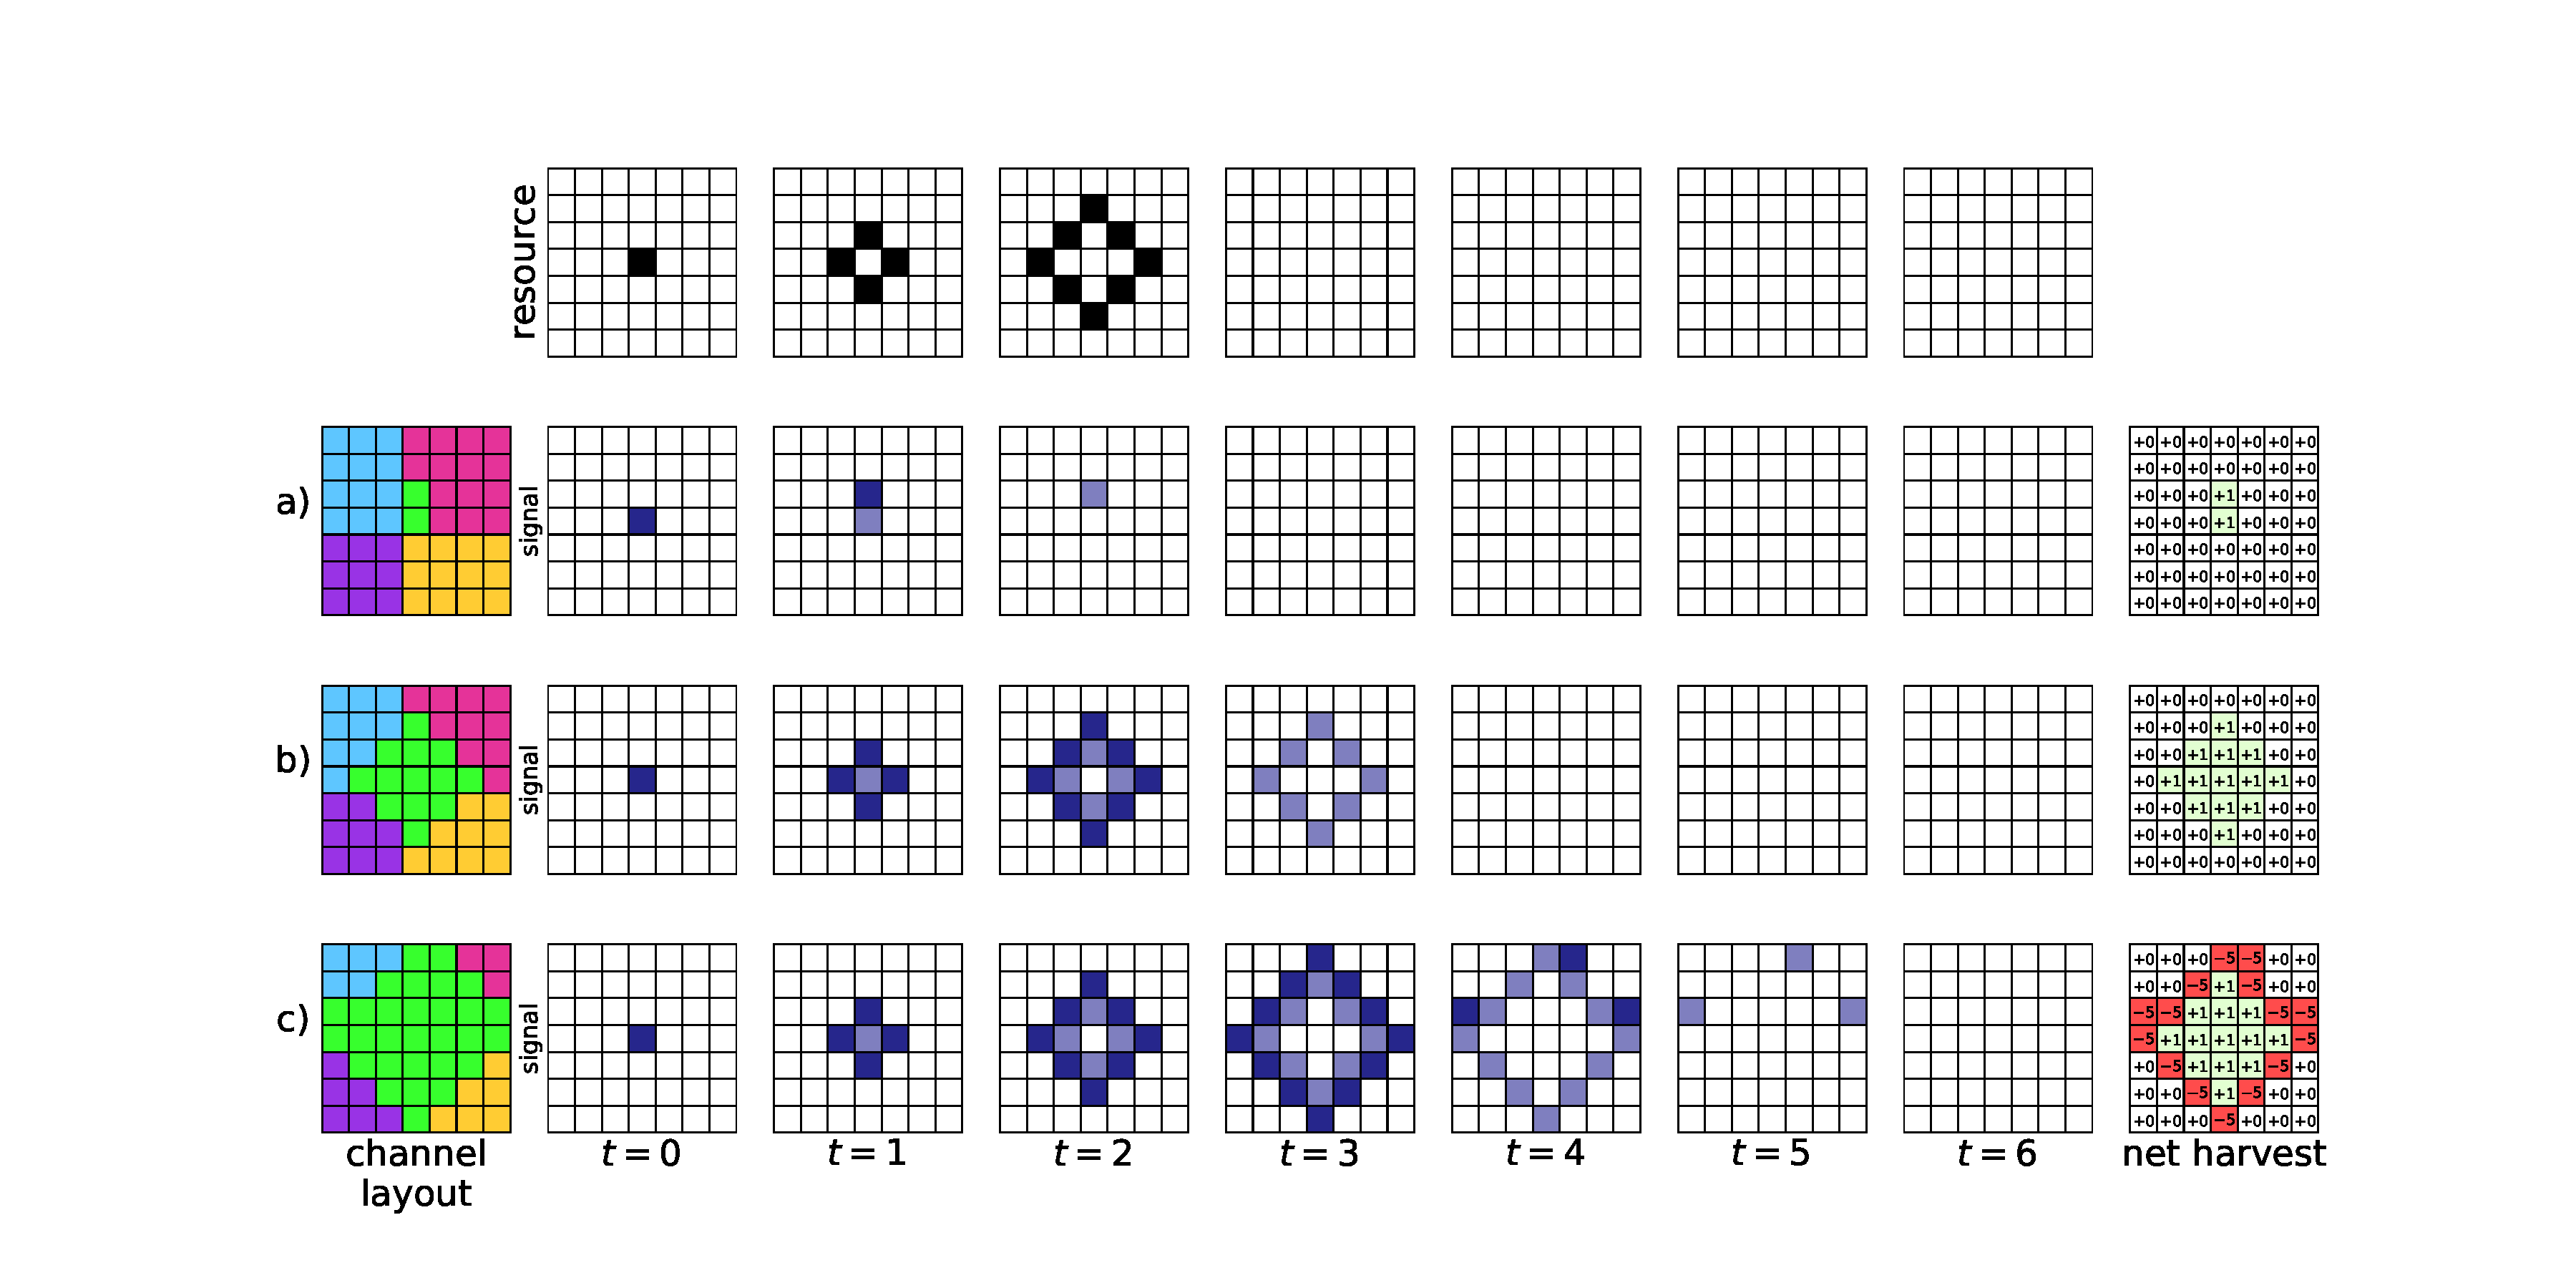
\includegraphics[width=2.0\columnwidth]{img/explanatory}
\caption{
Activation-quiescence signaling, and net resource collection for three different channel configurations during a single resource wave event.
At the top, a resource wave is depicted propagating over three updates and then ceasing for four updates (left to right).
In row $a$, an induced activation-quiescence signal tracking the resource wave yields a small net resource harvest (far right) to a small channel-signaling group.
In row $b$, a high net resource harvest is yielded to an intermediate-sized channel-signaling group.
Finally, in row $c$, a large channel-signaling group incurs a net negative resource harvest.
In rows $a$, $b$, and $c$, dark purple indicates the active state, light purple indicates the quiescent state, and white indicates the ready state.
}
\label{fig:explanatory}
\end{center}
\end{figure*}
